\documentclass[convert={density=300,outext=.png}]{standalone}
\usepackage{tikz}
\usetikzlibrary{shapes,arrows,decorations,decorations.pathmorphing,arrows.meta,patterns,decorations.markings}

\begin{document}
%% Use \usepackage{tikz}
%% Use \usetikzlibrary{shapes,arrows,decorations, decorations.pathmorphing,arrows.meta,patterns}
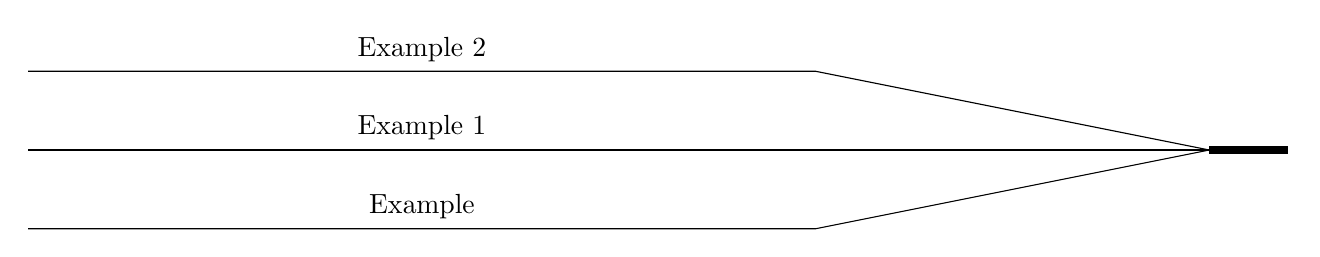
\begin{tikzpicture}[scale=1.0000]
	\tikzstyle{every node}=[scale=1.0000]
	
	%%Created with tikzpy
	
	\draw  (1.0000,1.0000,1.0000) -- (11.0000,1.0000,1.0000) -- (16.0000,2.0000,1.0000);
	\node [above ,align=left]  at (6.0000,1.0000,1.0000)  {Example};
	\draw  (1.0000,2.0000,1.0000) -- (11.0000,2.0000,1.0000) -- (16.0000,2.0000,1.0000);
	\node [above ,align=left]  at (6.0000,2.0000,1.0000)  {Example 1};
	\draw  (1.0000,3.0000,1.0000) -- (11.0000,3.0000,1.0000) -- (16.0000,2.0000,1.0000);
	\node [above ,align=left]  at (6.0000,3.0000,1.0000)  {Example 2};
	\draw [line width = 3.0000]  (16.0000,2.0000,1.0000) -- (17.0000,2.0000,1.0000);

\end{tikzpicture}
\end{document}
